%%%%%%%%%%%%%%%%%%%%%%%%%%%%%%%%%%%%%%%%%%%%%%%%%%%%%%%%%%%%%%%
%% HKUST Thesis LaTeX Template
%%
%% Check the project website for latest updates:
%% https://github.com/HKFoggyU/hkust-thesis
%%
%% Contributors:
%% https://github.com/HKFoggyU/hkust-thesis/graphs/contributors
%% 
%% License:
%% LaTeX Project Public License (version 1.3c)
%%
%%%%%%%%%%%%%%%%%%%%%%%%%%%%%%%%%%%%%%%%%%%%%%%%%%%%%%%%%%%%%%%

%% Pass options to loaded packages in `.cls` file:
% \PassOptionsToPackage{separate-uncertainty=true, separate-uncertainty-units=single}{siunitx}

%% The following option is to set hyperref colors for preview,
%% but commented by default for submission and printing
% \PassOptionsToPackage{colorlinks=true,urlcolor=blue,citecolor=red,anchorcolor=blue}{hyperref}

%% The following option is to display the full name of the authors.
%% It comes with the setting to display the full author names in the List of Publications
\PassOptionsToPackage{giveninits=false}{biblatex}

\documentclass[
  %customlatinfont = windows,
  %custombibstyle = nature,
  displaycommittee = false,
  % blankpage = true,
]{hkustthesis}

%% Thesis information
\hkustsetup {
  %% Please wrap the items with {}.
  %% If one item is not applicable, just leave it {}.
  %% Please do not leave any blank lines without {}.
  info = {
    degree        = {phd},  %% phd / mphil
    title         = {Triggering\texorpdfstring{\\}{}the Forth Impact},
    keywords      = {Neon, Genesis, Evangelion},
    author        = {Cruel Angel},
    school        = {School of SEELE},
    department    = {Department of NERV},
    program       = {Human Instrumentality},
    major         = {},
    supervisor    = {Prof. Adams},
    %% Co-supervisor; leave it {} if not available
    co-supervisor = {Prof. Lilith},
    submit-month  = {August 2021},      % <month year>
    submit-date   = {13 August 2021},   % <date month year>
    defend-date   = {8 March 2021},     % <date month year>
    depthead      = {Prof. Ikari Yui, Head of Department},
    %% reviewers only for some departments, like ECE
    reviewer      = {Prof. AAA (Chairperson), 
                     Prof. BBB (Supervisor),
                     Prof. CCC (Co-Supervisor),
                     Prof. DDD,
                     Prof. EEE,
                     Prof. FFF},
    reviewerdept  = {Department of Electronic and Computer Engineering,
                     Department of ECE,
                     Department of ECE,
                     Department of ECE,
                     Department of ECE,
                     Department of Physics},
    reviewerext   = {Prof. FFF (External Examiner),
                     Department of HH\\{University of UU, at VV}},
    % reviewerext   = {},
    city          = {Geo Front},
  }
}

%% Import extra packages
% \usepackage{indentfirst, xspace, xcolor}

%% Add custom command
% \newcommand{\todo}[1]{\textcolor{red}{TODO: #1}}
\newcommand{\eg}{\textit{e.g.}, }
\newcommand{\ie}{\textit{i.e.}, }

%% Set the specific author in bold style.
%% See https://tex.stackexchange.com/a/304968
%% Need to set `author+an = {n=highlight}` for your n-th authorship in bib file.
%% See more examples in the PDF manual.
\renewcommand*{\mkbibnamegiven}[1]{\ifitemannotation{highlight}{\textbf{#1}}{#1}}
\renewcommand*{\mkbibnamefamily}[1]{\ifitemannotation{highlight}{\textbf{#1}}{#1}}
%% The bib file for `List of Publications`
\addbibresource{mythesis_LoP.bib}

%% Import bib file for bibliography
\addbibresource{mythesis.bib}

\begin{document}

%% -------------------------------------------------
%% Thesis structure: In the order of
%% -------------------------------------------------
%% Titlepage  -> Authorization -> Signature ->
%% Acknowledgements ->
%% TOC -> List of Figures -> List of Tables ->
%% Abstract -> 
%% -------------------------------------------------
%% <Main body> -> 
%% -------------------------------------------------
%% References -> (Appendices)
%% -------------------------------------------------

\frontmatter
\maketitle 

\authorization
\signaturepage

\begin{acknowledgements}

Thank you, all the Evangelion.

\end{acknowledgements}


\tableofcontents
\listoffigures
\listoftables
% TODO: see \cmd{\newlistofalgorithms}
\newlistofalgorithms % This is to maintain the same appearance

%% Dedication and Preface are optional
%\begin{dedication}
  Dedicated to someone like you.
\end{dedication}

%\begin{preface}

\blindtext

\begin{flushright}
Author\\
2021. HK
\end{flushright}

\end{preface}

\begin{abstract}
\blindtext

\blindtext
\end{abstract}


%% -------------------------------------------------
%% Main body
%% -------------------------------------------------
\mainmatter

\chapter{Introduction}\label{chap:introduction}

\section{Background}\label{chap:intro:sec:background}

\blindtext

Cite a paper \cite{test}. \cref{chap:sample} will give more examples.

\subsection{Enumitem}

Itemize.

\begin{itemize}
  \item Test test.
  \item Test test.
  \item Test test.
  \begin{itemize}
    \item test test
    \item test test\footnote{\blindtext}
    \item test test
    \item test test
  \end{itemize}
  \item Test test.
\end{itemize}

Enumerate.

\begin{enumerate}
  \item Test test.
  \item Test test.
  \item Test test.
  \begin{enumerate}
    \item test test
    \item test test\footnote{\blindtext}
    \item test test
    \item test test
  \end{enumerate}
  \item Test test.
\end{enumerate}


\chapter{Example chapter}\label{chap:sample}

\section{Background}\label{chap:intro:sec:background}

\blindtext

Cite a paper \cite{test}. \cref{chap:sample} will give more examples.

\subsection{Enumitem}

Itemize.

\begin{itemize}
  \item Test test.
  \item Test test.
  \begin{itemize}
    \item test test
    \item test test\footnote{\blindtext}
    \item test test
  \end{itemize}
  \item Test test.
\end{itemize}

Enumerate.

\begin{enumerate}
  \item Test test.
  \item Test test.
  \begin{enumerate}
    \item test test
    \item test test\footnote{\blindtext}
    \item test test
  \end{enumerate}
  \item Test test.
\end{enumerate}

\section{Math}

\subsection{Symbols}

\begin{itemize}
  \item Calligraphic letters: $\mathcal{A}$ 
  \item Mathbb letters: $\mathbb{A}$
  \item Mathfrak letters: $\mathfrak{A}$
  \item Math Sans serif letters: $\mathsf{A}$
  \item Math bold letters: $\mathbf{A}$
  \item Math bold upright Greek letters: $\mathbf{\alpha}$ (Not displaying! Use the following one.)
  \item Math bold upright Greek letters: $\symbfup{\alpha}$
  \item Math bold italic Greek letters: $\bm{\alpha}$
  \item Math bold italic Greek letters: $\mathbi{A}$
\end{itemize}

Avoid using \lstinline|bm| package as it conflicts with \lstinline|unicode-math| and it is outdated for \hologo{XeLaTeX}.
You can alias some math commands by \lstinline|\newcommand| or \lstinline|\renewcommand| anyway.

\subsection{Equations}

\begin{equation}
  E^2 = m^2 + p^2\label{eq:mass-energy}
\end{equation}

You can use \lstinline|\cref{}| to automatically setup the cross reference name; instead, you can always use \lstinline|\ref{}| to customize the appearance of the cross reference.

\cref{eq:mass-energy} or Equation (\ref{eq:mass-energy}) gives the mass-energy relationship.

\subsection{Theorem}

\begin{definition}
  LCL is orange juice.
\end{definition}

\begin{proof}
  They are both orange.
\end{proof}

\begin{algorithm}[htbp]
  \caption{Temp}
  \begin{algorithmic}[1]
    \STATE Temp
  \end{algorithmic}
\end{algorithm}

Available theorem environments are listed below:

algorithm, assumption, axiom, conclusion, condition, corollary, definition, example, lemma, proof, property, proposition, remark, theorem.


\section{Figure}
An example image is shown in \cref{fig:tikz example} or Figure (\ref{fig:tikz example}).

\begin{figure}[H]
  \centering
  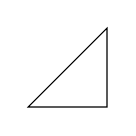
\begin{tikzpicture}
    \draw (0,0) -- (1, 0) -- (1, 1) -- cycle;
  \end{tikzpicture}
  \caption{An example tikz picture with a short caption.}
  \label{fig:tikz example short}
\end{figure}

\begin{figure}[H]
  \centering
  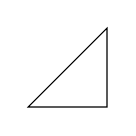
\begin{tikzpicture}
    \draw (0,0) -- (1, 0) -- (1, 1) -- cycle;
  \end{tikzpicture}
  \caption{An example tikz picture with long caption and breakline\\\blindtext}
  \label{fig:tikz example}
\end{figure}

\section{Table}

An example table is shown in \cref{tab:environment} or Table (\ref{tab:environment}).

\begin{table}[H]
  \centering
  \caption{A table with a short caption.}
  \label{tab:table_short}
  \begin{tabular}{lll}
    \toprule
    OS & TeX & Test \\
    \midrule
    Overleaf                 & \hologo{TeX}\,Live 2021/2/3    & Pass \\
    Windows 10               & \hologo{TeX}\,Live 2020        & \color{red}{\verb|ltxhook| problem} \\
    Ubuntu 20.04             & \hologo{TeX}\,Live 2021        & Pass \\
    \bottomrule
  \end{tabular}
\end{table}

\begin{table}[H]
  \centering
  \caption{Test result on different platforms with long caption and breakline\\\blindtext}
  \label{tab:environment}
  \begin{tabular}{lll}
    \toprule
    OS & TeX & Test \\
    \midrule
    Overleaf                 & \hologo{TeX}\,Live 2021/2/3    & Pass \\
    Arch Linux (2023.11)     & \hologo{TeX}\,Live             & Pass \\
    Windows 10/11            & \hologo{TeX}\,Live 2021        & Pass \\
    macOS 10.15              & \hologo{TeX}\,Live 2021        & Pass \\
    Windows 10               & \hologo{TeX}\,Live 2020        & \color{red}{\verb|ltxhook| problem} \\
    Ubuntu 20.04             & \hologo{TeX}\,Live 2021        & Pass \\
    Termux                   & \hologo{TeX}\,Live 2021        & Pass \\
    Windows 11               & \hologo{MiKTeX} 4.9            & Pass \\
    Windows 10               & \hologo{MiKTeX} 4.4            & Pass \\
    \bottomrule
  \end{tabular}
\end{table}


\section{Code}

\subsection{Inline code}
Use \lstinline$\lstinline|<code>|$ to print code snippets. The \lstinline$||$ marks delimit
the code and can be replaced by any character not in the code;
\textit{e.g.}   \lstinline|\lstinline$<code>$| gives the same result.

\subsection{Code environment}
The code to draw the \cref{fig:tikz example} is listed below:
\begin{lstlisting}[caption={\hologo{LaTeX} code for inserting a figure}]
\begin{figure}[htb]
  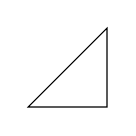
\begin{tikzpicture}
    \draw (0,0) -- (1, 0) -- (1, 1) -- cycle;
  \end{tikzpicture}
  \caption{An example picture with long caption: \blindtext\\\blindtext}
  \label{fig:tikz example} % this is a comment
\end{figure}
\end{lstlisting}

\section{Manage citations}
\label{chap:bibliography}

Use \lstinline|biber| as \hologo{BibTeX} backend.

\subsection{Add and manage}

Entries are stored in \lstinline|mythesis.bib|. For other sources, modify following commands in \lstinline|mythesis.tex|:
\begin{lstlisting}[language=TeX]
\addbibresource{mythesis.bib}
\end{lstlisting}

\subsection{Citation style}

As described in the sample page from ECE department, the style is set to \lstinline|ieee|. You can modify the style in the \lstinline|hkustthesis.cls| file as you wish.

\chapter{Conclusions}
\label{chap:conclusions}

\blindtext


%% -------------------------------------------------
%% References
%% -------------------------------------------------

\printbibliography[heading=bibintoc,title=References]

%% -------------------------------------------------
%% Appendices
%% -------------------------------------------------
\appendix

\chapter{List of Publications}
% "List of Publications" citations can be stored in `mythesis.bib` or,
% another bib file, remember to add its name in `\addbibresource{}`

% Journal Publications
\paperlist[Journal Publications]{ChaiACSNano2022,HermanNature2007,WarrenSci.Adv.2022}

% Conference Publications
\paperlist[Conference Publications]{LuConf.LasersElectro-Opt.2021Pap.SW3B12021, JehleImagingAppl.Opt.20162016Pap.IM4F22016}

% You can add customized title name in the []

\chapter{FYTGS Requirements}
\label{chap:thesis-preparation}

The requirements are from the \href{https://rpghandbook.hkust.edu.hk/appendices-guidelines-on-thesis-preparation}{RPG Handbook}.

\section{Components}

Order. A thesis should contain the following parts in the order shown:

\begin{enumerate}
  \item Title page, containing in this order:
    \begin{enumerate}
      \item thesis title
      \item full name of the candidate
      \item degree for which the thesis is submitted
      \item name of the University, \emph{i.e.} The Hong Kong University of Science and Technology
      \item month and year of submission
    \end{enumerate}
  \item Authorization page
  \item Signature page
  \item Acknowledgments
  \item Table of contents
  \item Lists of figures and tables
  \item Abstract ($\leq$ 300 words.)
  \item Thesis body
  \item Bibliography
  \item Appendices and other addenda, if any.
\end{enumerate}

\section{Language, Style and Format}

\subsection{Language}
Theses should be written in English.\\
Students in the School of Humanities and Social Science who are pursuing research work in the areas of Chinese Studies, and who can demonstrate a need to use Chinese to write their theses should seek prior approval from the School via their thesis supervisor and the divisional head.\\
If approval is granted, students are also required to produce a translation of the title page, authorization page, signature page, table of contents and the abstract in English.

\subsection{Pagination}

\begin{enumerate}
  \item All pages, starting with the Title page should be numbered.
  \item All page numbers should be centered, at the bottom of each page.
  \item Page numbers of materials preceding the body of the text should be in small Roman numerals.
  \item Page numbers of the text, beginning with the first page of the first chapter and continuing through the bibliography, including any pages with tables, maps, figures, photographs, etc., and any subsequent appendices, should be in Arabic numerals.
  \item Start a new page after each chapter or section but not after a sub-section.
\end{enumerate}

\emph{Note: That means the Title page will be page i; the first page of the first chapter will be page 1.}

\subsection{Format}

\begin{enumerate}
  \item A conventional font, size 12-point, 10 to 12 characters per inch must be used.
  \item One-and-a-half line spacing should be used throughout the thesis, except for abstracts, indented quotations or footnotes where single line spacing may be used.
  \item All margins—top, bottom, sides—should be consistently 25mm (or no more than 30mm) in width. The same margin should be used throughout a thesis. Exceptionally, margins of a different size may be used when the nature of the thesis requires it.
\end{enumerate}

\subsection{Footnotes}

\begin{enumerate}
  \item Footnotes may be placed at the bottom of the page, at the end of each chapter or after the end of the thesis body.
  \item Like references, footnotes should be presented in a standard format appropriate to the discipline.
  \item Both the position and format of footnotes should be consistent throughout the thesis.
\end{enumerate}

\subsection{Appendices}

The format of each appended item should be consistent with the nature of that item, whether text, diagram, figure, etc., and should follow the guidelines for that item as listed here.

\subsection{Figures, Tables and Illustrations}

Figures, tables, graphs, etc., should be positioned according to the scientific publication conventions of the discipline, e.g., interspersed in text or collected at the end of chapters. Charts, graphs, maps, and tables that are larger than a standard page should be provided as appendices.

\subsection{Photographs/Images}

\begin{enumerate}
  \item High contrast photos should be used because they reproduce well. Photographs with a glossy finish and those with dark backgrounds should be avoided.
  \item Images should be dense enough to provide 300 ppi for printing and 72 dpi for viewing.
\end{enumerate}

\subsection{Additional Materials}

Raw files, datasets, media files, and high resolution photographs/images of any format can be included.

\emph{Note: Students should get approval from their department head before deviating from any of the above requirements concerning paper size, font, margins, etc. }


\end{document}
